\documentclass{amsart}

\usepackage{graphicx}
\usepackage{parskip}
\usepackage{latexsym}
\usepackage{amsfonts}
\usepackage{amssymb}
\usepackage{amsmath}
\usepackage{amscd}
\usepackage{eucal}
\usepackage[all]{xy}
\usepackage{pstricks}
\usepackage{tabularx}
\newcommand{\bs}{\boldsymbol}
\newcommand{\mb}{\mathbf}
\renewcommand{\dot}{\centerdot}


\title{Flipped teaching as a method for engaging large groups}
\author{Dr Sam Marsh}
\author{Dr Nick Gurski}


\begin{document}
\maketitle

\begin{abstract}
In a large-scale trial at the University of Sheffield ($n=236$), we implemented a flipped approach to teaching mathematics to first-year engineers. Lectures were discontinued and replaced with an integrated format of specially filmed short videos, online quizzes and twice as much small-group learning.  We found strong evidence that engagement and exam performance were boosted by the new method by comparing with students on an identical syllabus taking the same exam but taught traditionally.
\end{abstract}

\section{Introduction}

\subsection{Background}

The School of Mathematics and Statistics provides mathematics teaching for undergraduate students in the Faculty of Engineering at the University of Sheffield. Predominantly, these modules have been taught in a traditional format of two large-group lectures (200 students or more) and one smaller-group problem class (approximately 40 students) per week.  Attendance records are kept for problem classes but not lectures.  We find that attendance usually starts high, but drops off as time progresses (see Figure 1).

\begin{center}
\begin{figure}[hbt]
\includegraphics[bb=50 250 562 545,width=1\textwidth]{Figure1.pdf}
\caption{Problem class attendance on two traditionally taught engineering mathematics modules, Semester 1 2013--14}
\end{figure}
\end{center}

A working group was established to look into the effectiveness of these modules, with a particular focus on whether a flipped approach, based around videos, online tests and small-group classes, could provide a more engaging course for students.

The working group established a key proposal: that large-group lectures would be discontinued, and their content split into theory (to be included in the videos) and examples (to be done in classes).  Further, the amount of contact time allocated to small-group learning would be doubled.  This approach was to be piloted on a first-year module of 236 students, with two other modules totalling 298 students which cover an identical syllabus but taught traditionally used as a comparison.

\subsection{Literature}%I suggest we put a couple of paragraphs about flipped learning here, no more, and not too dense.





%This is some stuff I have copied from my CiLT 2 portfolio, we can include or not.
%
%The teaching that goes on in the old MAS140/151/152 was very task-oriented:  the lecturer would outline a range of tasks the students would be asked to perform, and then give them explicit tools for performing those tasks.  This is a level of teaching that is concerned primarily with \textit{execution} rather than \textit{theory}; here the focus was on learning particular methods and not the theory that gives rise to those methods.  Now, there was some theory presented in this module, but that theory was not the top priority for either lecturer or student. Thus this teaching was really about \textit{problem-solving}, and not about \textit{problem-understanding}.  While from some perspectives this might seem shallow, it is appropriate, given the audience, for at least two reasons:  first, on the whole, engineering students respond well to the idea of solving specific problems and getting an answer, and second, the module is intended to prepare them to solve the kinds of problems that will come up during their engineering degree.
%
%In practice, this means that the there were two primary learning activities.  The first was the lecture, of which there are two per week, and these lectures were executed in an entirely traditional fashion.
%%First, material was introduced.  This would include explaining what kinds of problem we were going to solve, and perhaps a bit of theory that would point us in the right direction for a solution.  Sometimes this theory would actually get us all the way to the correct solution method, sometimes there would be a substantial gap between theory and solution or even no justification at all for how the background theory would produce the solution method given.  After explaining how to work a kind of problem in the abstract, examples would be explained; these would increase in difficulty or effort required, and would give the students a feeling for what they might expect later.  I made some small adjustments to the lectures, most notably adding in questions for the students to work during the lecture itself.  These problems, often broken into small steps, allow me to get a good feel for what students are understanding or not understanding, and I feel like this change has been quite successful.
%The second learning activity was the weekly tutorial sessions.  Each student was assigned to a tutorial group, and a group was usually about 20-30 students per staff member or postgraduate assistant; thus some tutorials would have 40 students with one staff member and one assistant, while others would have 80 students with one staff member and three assistants.  These tutorials are ``mandatory'' in the sense that we claimed they were, but this was not enforced explicitly.  Attendance was kept, and we often correlated poor attendance with poor performance, but beyond that very little was usually done with this information.  Attendance numbers would usually start quite high, but then drop off as time progressed.
%%We do sometimes get specific feedback on student questionnaires about the tutorials, and it usually takes one of a few standard forms:  the tutorials were helpful, my tutor was helpful, or my tutor was not helpful.  I do not recall seeing questionnaires in which students reported that the tutorials themselves were not helpful, although the decline in attendance does indicate that they lack interest in the tutorials even if they find them beneficial.
%
%%While the activities during any given tutorial are largely up to the staff member running that tutorial (who is usually not the lecturer, given the size of these modules), it is safe to say that the primary activity during tutorials is working on questions from tutorial sheets that the lecturer provides in advance.  Students tend to approach these problem sheets in one of two ways.  The first approach is to do every problem, in order, regardless of how far behind you get.  The second approach is to work on the sheet which claims to be for that week in the lecture, regardless of how the material on the sheet actually corresponds to the lecture material.  All of this, in addition to the differences in the personalities and teaching styles of the tutors and assistants involved, results in a large degree of variation in learning that goes on in tutorial sessions.  If a student actively seeks out assistance on relevant problems and generally follows along with the lecture so that they are attempting appropriate problems, then this system can work very well.  For less engaged students, particularly with a shy member of staff leading the tutorial, this can easily turn into an hour of gossiping with friends or staring blankly at problems without making any progress at all.
%
%For many of these modules, feedback for students was somewhat limited.  In one case (MAS153) there were a few marked homework assignments, but for many of the modules there was nothing as direct as an assessed piece of work during the semester, simply due to class sizes and available resources.  Many students sought feedback during the weekly tutorials, and others would attend lecturer office hours, but both of these methods only provided feedback if the students took the initiative. % Students do bring up the topic of feedback on occasion in their questionnaires, but remarks on the topic are by no means ubiquitous.  One of the main reasons that so many of these modules do not have feedback such as marked homework is simple economics -- as these tend to be large modules, it requires a considerable amount of work just to mark a single short assignment from each student.  These kinds of economic issues influence many factors in our engineering teaching, and going forward SoMaS should bear in mind both economics and quality-of-teaching issues when looking to improve our modules for engineers.
%Assessment, then, was largely or entirely by exam.  In previous years, this would involve one exam each semester, but our Engineering Faculty changed all of their modules to only having a single exam after Semester 2 and thus we had a single, 3-hour exam covering all of the material from the entire year.  The contents of this exam were split evenly between material from the first and second semesters, and we kept a similar format as in previous exams.  When changing from two exams to a single exam, results were far worse than in past years; the mean dropped dramatically, to the point where we were essentially forced to scale up the exams for the first time in years.  Note, however, that there were not particularly clear trends indicating that students were not understanding certain topics, rather that they performed poorly throughout the exam.
%
%Up until exams, this cohort seemed roughly similar to previous years' in terms of ability, background, and motivation.  Assessing only once at the end of the year instead of each semester seemed to have a noticeable impact on how students approached learning the mathematics involved.  At one Engineering exam board meeting, it was suggested that these low exam results are perhaps more in line with the students' actual learning than in the past, the hypothesis being that students tended to put off doing any work during the semester, leaving it all until right before an exam.  Students were unlikely to retain any real understanding of the mathematics involved, but with only a single semester's worth of material they were able to pass an exam.
%
%End history of engineering teaching, begin some random theory I found
%
%Williams  makes the argument in \cite{w} against the ``final exam'' as the ultimate means of assessment, bringing up how this method can lead to very shallow learning, and we certainly believe that this phenomenon contributed to the poor exam performance we witnessed.  This brings up an important consideration, namely how to get students engaged with the material over the entire year even though the exam is not until May.  In \cite{e}, Elton considers student motivation from the perspective of a motivational theory of work pioneered by Herzberg.  One conclusion to draw from this research is that poor student motivation can result from the poor management of extrinsic and intrinsic motivating factors.  In particular, Elton discusses how students often are positively motivated by being able to show off achievement throughout the learning experience, and the focusing on a single exam can change the motivator of ``academic achievement'' from a positive motivator to a negative one by overly stressing failure instead of rewarding success.
%
%Next paragraph doesn't seem useful:
%
%Golden and Stripp describe a teaching situation at the University of West England in \cite{gs} which was similar to ours in Sheffield.  They discuss a first year mathematics module for Engineering students coming from a wide range of programmes, and outline a teaching strategy that is very similar to our current one with a single important difference.  Their module consisted of two hours of lecture per week, and one hour of tutorial, just as ours did, and most materials for the module can be obtained directly by students from a website.  The main difference between their module and our Engineering modules is the use of routine computer testing.  The particular strategy used by those authors is to have online tests at the end of each ``Learning Unit'', and they say that generally means about every four weeks.  These online tests are generated randomly from a bank of appropriate questions, and are marked immediately once the student completes a test.  Each student has two weeks to complete their tests, and they may make three attempts in total, each one a new, randomly generated test; the highest mark is recorded, and this contributes a full 50\% to the final assessment of the module.
%
%A study \cite{nk} by Nguyen and Kulm looked at web-based practice and assessment tools in middle school (age 11-13) children.  These kinds of software will automatically produce mathematics problems of a particular type which students are  able to work, submit an answer and receive an immediate mark together with certain kinds of feedback.  %(As a note, this kind of online assessment is already being used in some modules in SoMaS.  Our own Neil Strickland wrote his own version of this kind of software which can randomly generate questions and then check student answers using the standard mathematics software Maple.)
%Students are able to repeat a certain kind of problem until they are comfortable, with new wording and random number values generated each time.  In this study, the children who worked with the computer-generated problems scored significantly higher than the children who continued working problems with pencil and paper in the classroom.  The process of getting immediate feedback helped the students correct errors and recognise common mistakes which they were then able to avoid in future work.
%
%It is important to remember that there is not necessarily a clear divide between online learning and traditional, face-to-face learning; any learning experience that has some duration could easily contain elements of both.  In many ways, online learning faces many of the same obstacles that face-to-face learning does.  One framework for studying the social learning experience is the Community of Inquiry model \cite{ga} which describes and explains three crucial features of a social learning environment:  social presence, teaching presence, and cognitive presence.  Students view teacher presence as very important in online education, and there is a correlation between the perceived learning by students and the quality and amount of teacher presence in the online learning environment \cite{jt}.  But this should not be a surprising result, as the same is true for face-to-face learning environments \cite{ra}.  Thus in many ways, studying online learning is done using the same methods and asking the same questions as one might in studying traditional educational methods.
%
%A study \cite{kwsc} done at the University of Alabama considered three groups of students taking a graduate-level mathematics course for engineers.  In this study, all three groups performed very similarly, with the students in the blended group outperforming those in the traditional group on exams and with students in the online-only group performing the best on analytical, take-home assessments.  For the first of these results, that authors suggest that students having access to both online and traditional methods will choose the method that best suits them, thus increasing overall performance.  For the results on the analytical assessments, the authors suggest that students in the online-only group were required to work harder and understand the material at a deeper level since they did not have easy access to an outside source of knowledge (i.e., the instructor) to supply hints or solutions immediately.

\section{Comparison of teaching methods}

\subsection{Summary}

The difference in structure of the flipped approach as compared with the traditional course format is summarised in Table 1.  Both formats are for year-long, 20-credit modules for first year engineers from varying departments studying the same syllabus.  Note that timetabled sessions are 50-minutes in duration, and these are the units used for counting lectures and problem classes.

\begin{table}[htb]
\begin{tabularx}{0.8\textwidth}{lXX}
 & Traditional & Flipped\\\hline
Lectures per week & 2 & 0\\
Problem classes per week & 1 & 2\\
Problem class format & Exercise booklet, reactive teaching & Worksheets, proactive teaching\\
Continuous assessment & End of semester homework & Online tests\\
Additional resources & Typed notes, office hour, webpage/VLE & Video lectures, typed notes, additional exercise booklet, discussion board, office hour, webpage/VLE
\end{tabularx}
\caption{Comparison of teaching formats}
\end{table}

The main differences in approach are that two or three short (10--15 minute) video lectures replace each face-to-face lecture, quick online tests follow each video, and problem classes are doubled in frequency and given more structure.

\subsection{Video delivery}

The videos are best described as for-purpose `chalk-and-talk' short films, made using minimal equipment (camcorder, lapel-mic, umbrella lights and blackboard in a standard office).  In a few places cutaways to narrated slides also feature.  The videos are hosted, unlisted, on Youtube and students access them as embedded into a page within the Assessment in Mathematics (AiM) learning-environment, itself mostly developed at our department.  AiM allows for each video to be followed by mathematical questions, randomly varied by student, and the underlying software is able to manipulate algebra so as to accept any valid rearrangement of a correct answer. It also gives instant feedback on student responses and records all activity, allowing us to track engagement and performance.

\subsection{Problem classes}

In a standard week students complete two iterations of the cycle: log in to AiM $>$ watch 3 videos $>$ rewatch if necessary $>$ complete the online tests $>$ attend a problem class. Additionally, students are encouraged to work on a booklet of practice exercises independently, supported by the course notes and staff or peers on an online discussion board.

Students are assigned to a problem class group of size 40.  These groups meet twice a week.  The class is run by a tutor who recaps and reinforces the theory seen in the videos (5--10 minutes), encourages input on an example demonstrated at the board (5--10 minutes), then sets problems for students to work on, encouraging peer-discussion.  Each problem class has a lesson plan which is made available subsequently to students via the course webpage.

The format for the new problem classes differs from our previous approach, where the ratio of teachers to students was better --- 40 students were catered for by one staff member and one postgraduate student assistant --- but the class was reactive, with students working on exercises and teaching staff responding to demand for assistance.


\section{Methodology}

The pilot implementation of our scheme was restricted to a module for one of the engineering departments (Module C, $n=236$), with modules for two further departments directly comparable (Module A, $n=137$, and Module B, $n=161$).  The latter two modules were lectured in a single group.  All students had attendance recorded at problem classes and received feedback questionnaires at the end of each semester.  Data on the use of the video-system (AiM) was recorded for students on Module C.  The exam was identical for all students and sat concurrently.

Raw exam data for the preceding two years was also available, where all three modules were taught in the traditional format with a common exam, allowing for an analysis of exam performance that could control for variations in the relative abilities of students on different courses.

\section{Analysis}

\subsection*{Engagement}

Attendance at problem classes was considerably better across the year for the new format, Module C (see Figures 2 and 3, and Table 2).  Students attended approximately three times as many problem classes across the year, due to a higher attendance rate ($77\%$ compared to $50$--$60\%$) over twice as many scheduled classes.

\begin{center}
\begin{figure}[hbt]
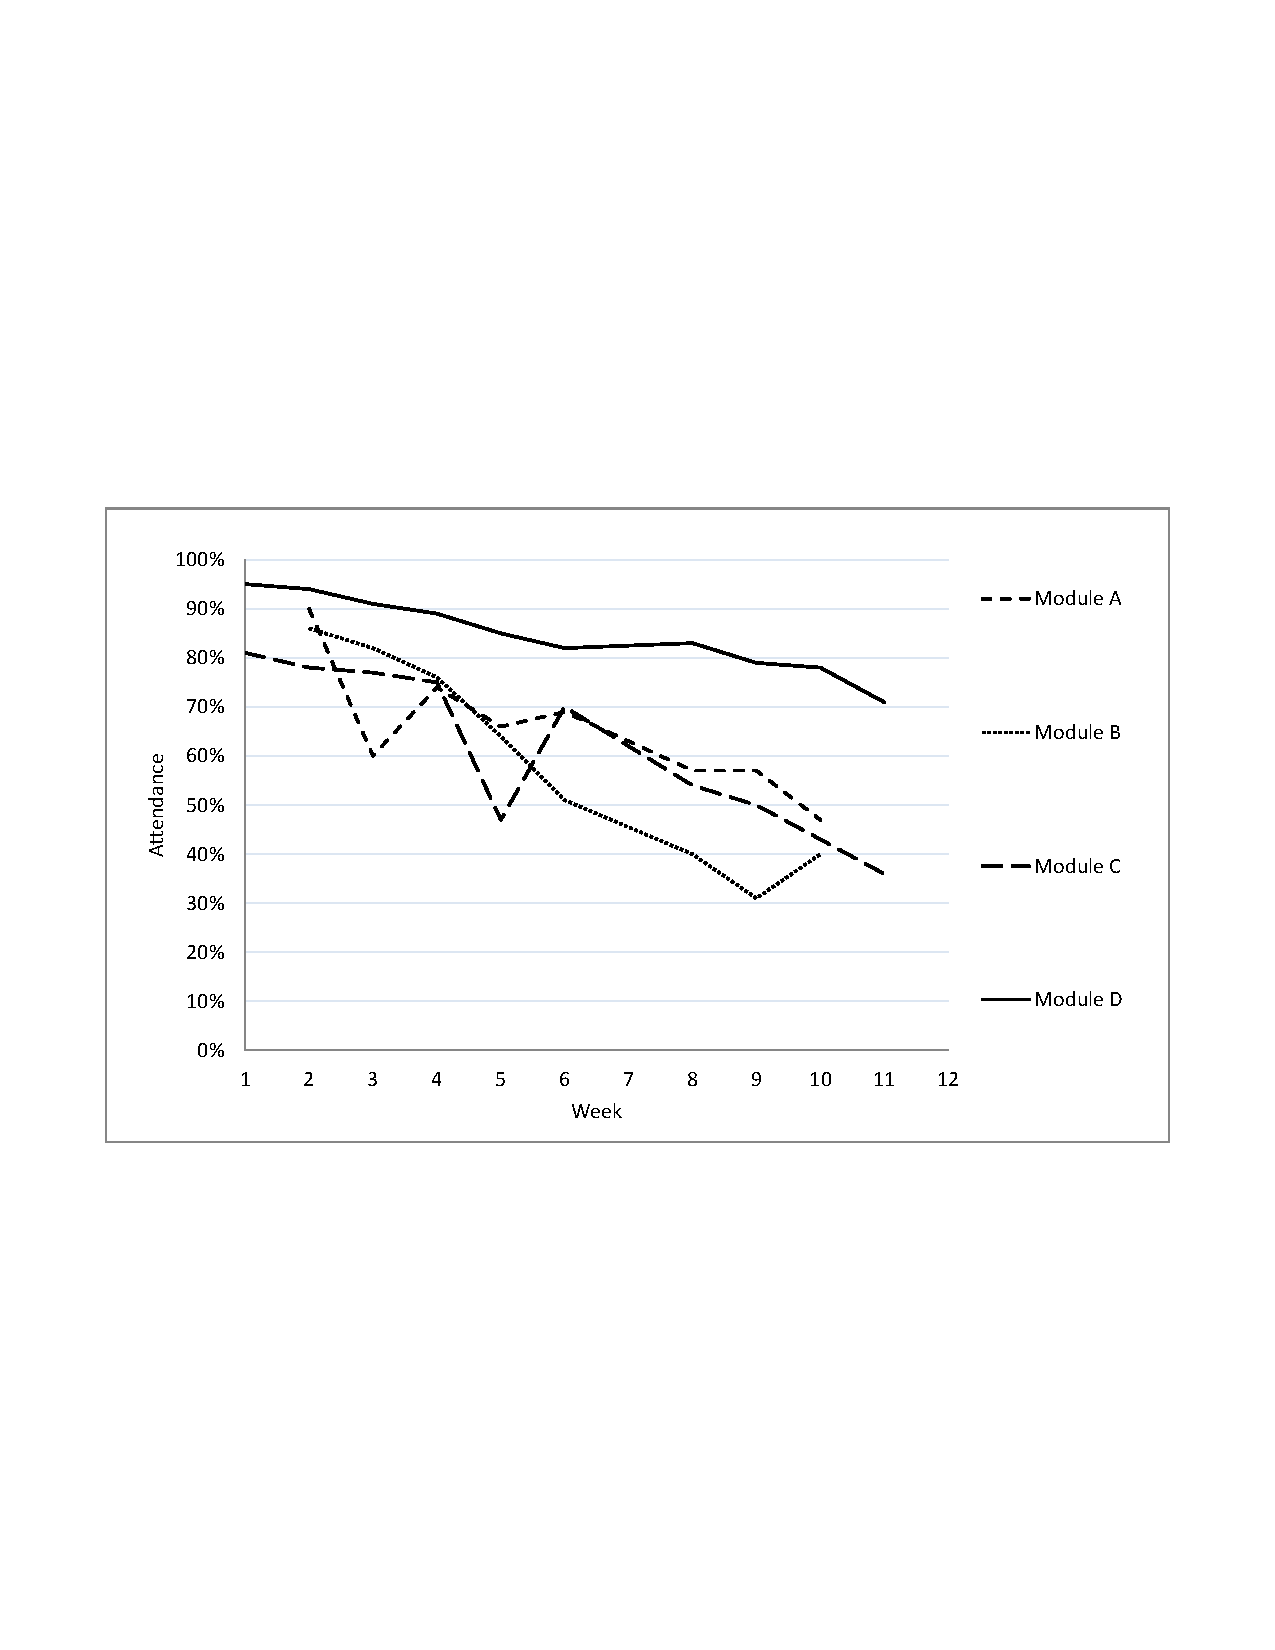
\includegraphics[bb=50 250 562 545,width=1\textwidth]{figure2.pdf}
\caption{Problem class attendance, Semester 1}
\end{figure}
\end{center}

\begin{center}
\begin{figure}[hbt]
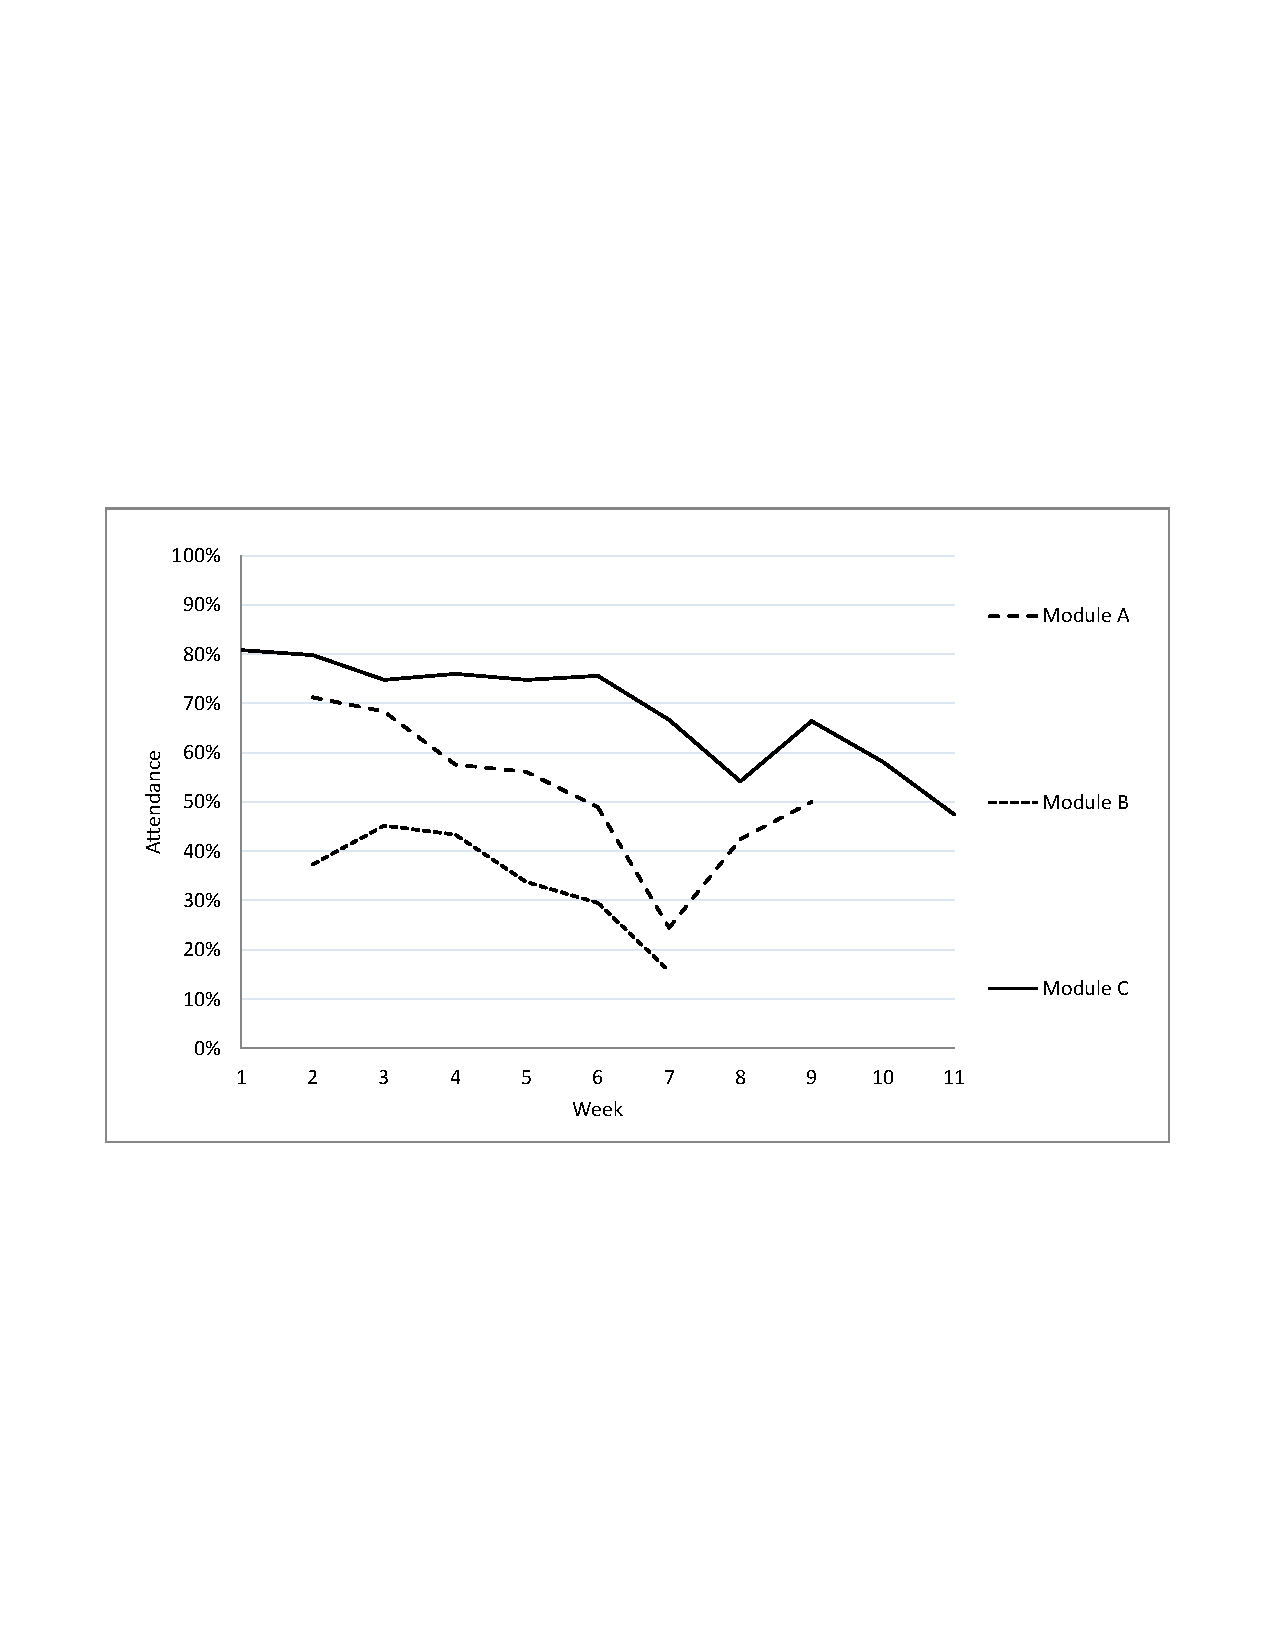
\includegraphics[bb=50 250 562 545,width=1\textwidth]{figure3.pdf}
\caption{Problem class attendance, Semester 2. Easter break occurred between Weeks 8 and 9.}
\end{figure}
\end{center}

\begin{table}[htb]
\begin{tabular}{lccc}
& Average attendance & Average no. classes attended\\\hline
Module A & 59\% & $10$--$12$*\\
Module B & 50\% & $7.5$--$11.5$*\\
Module C & 77\% & $31.5$
\end{tabular}
\caption{Summary of attendance data. The * indicates incomplete data towards the end of the course leading to the uncertainty shown.}
\end{table}

Additionally, as students were unable to access the online tests until they had watched the relevant video in full, without fast-forwarding, we were able to determine the number of students who had watched each video on time (see Figure 4).  The data from indicates that the vast majority of students (86\%) watched at least $80\%$ of the videos on time, and half of students watched at least $97\%$ of the videos on time.  It is possible, and indeed likely, that students who had not watched the videos on time watched them at a later date, but we didn't have a method for tracking such engagement.

\begin{center}
\begin{figure}[hbt]
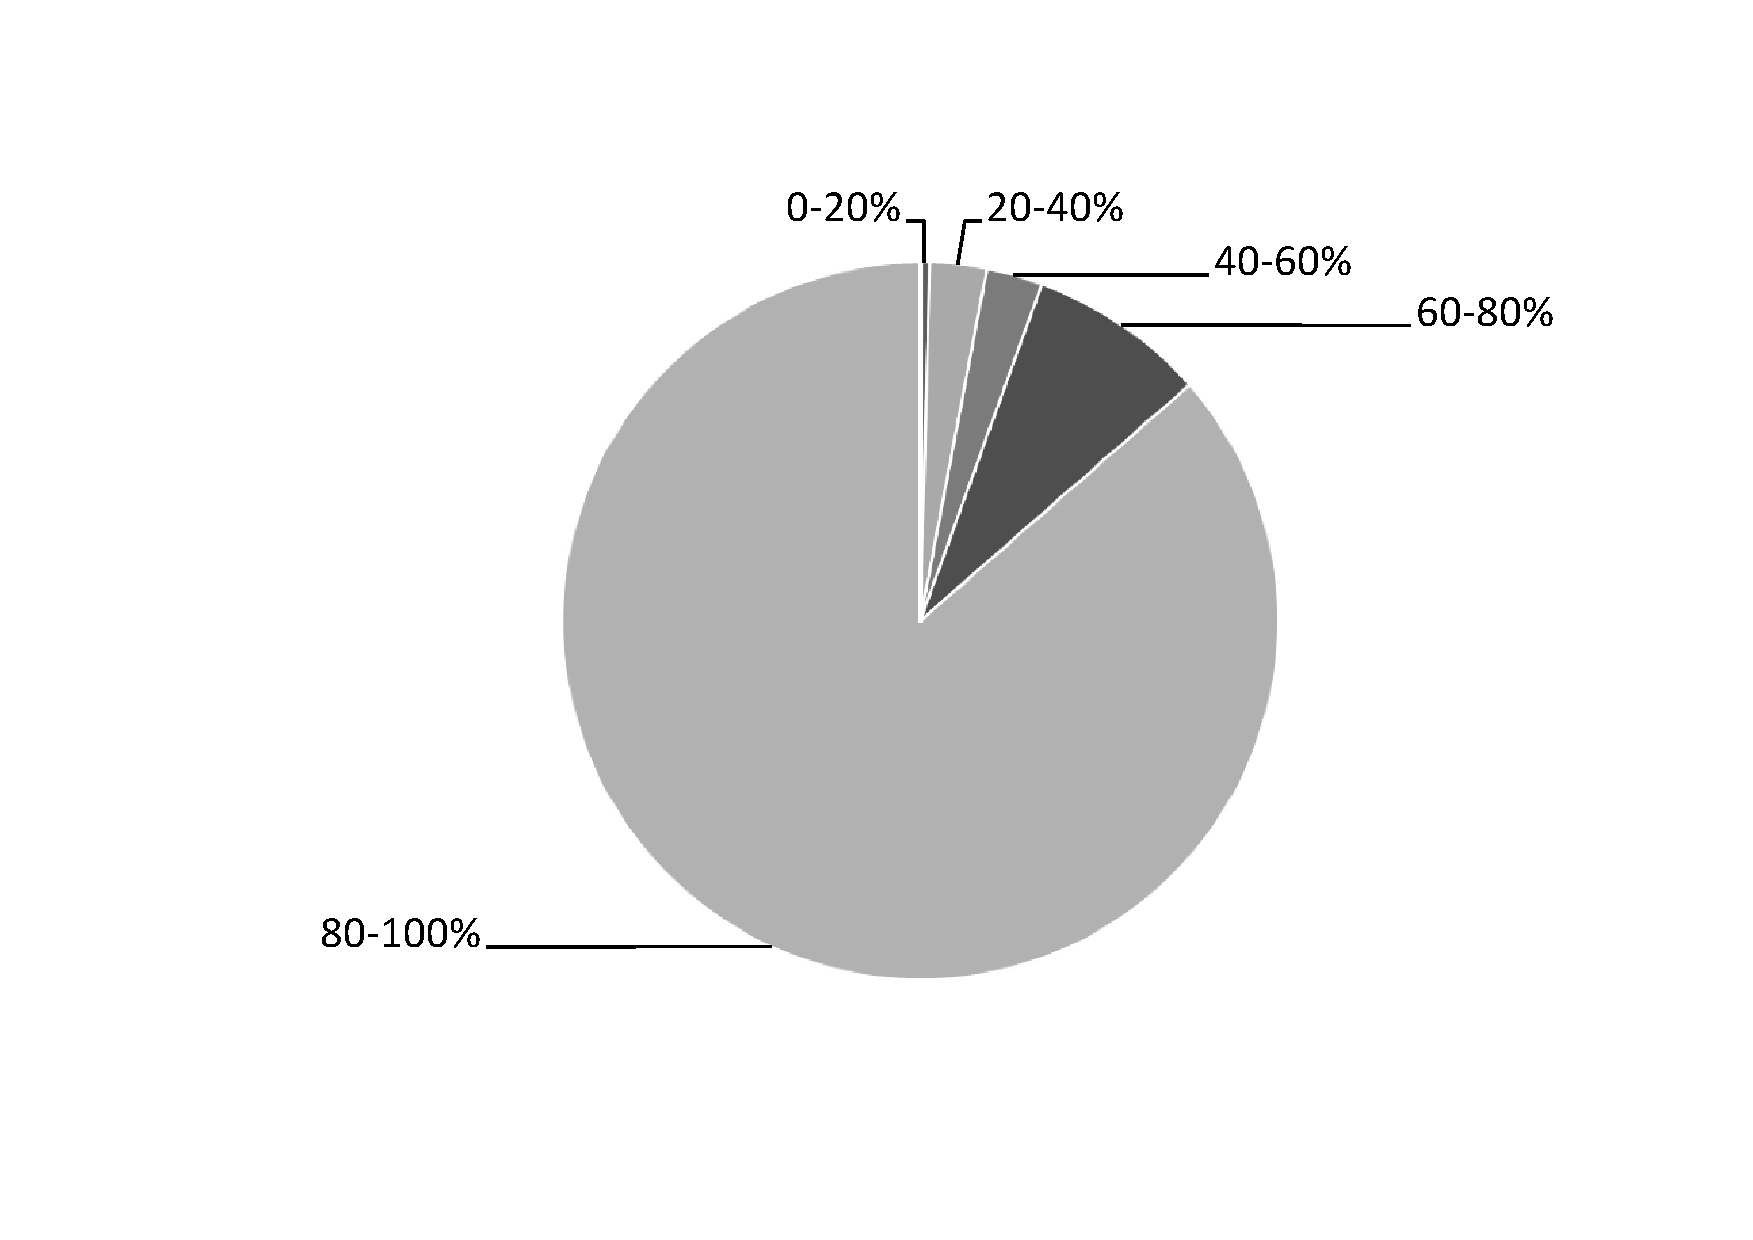
\includegraphics[width=1\textwidth]{figure4.pdf}
\caption{Proportions of videos watched on time}
\end{figure}
\end{center}

%\begin{table}[htb]
%\begin{tabular}{cc}
%Proportion watched on time & Number of students\\\hline
%0--20\% & 1\\
%20-40\% & 6\\
%40-60\% & 6\\
%60-80\% & 19\\
%80-97\% & 85\\
%97--100\% & 119
%\end{tabular}
%\caption{Proportion of videos watched on time (total number of students=236)}
%\end{table}

\subsection*{Student satisfaction}

Module feedback from students was very positive. In Semester 1, over 94.9\% were satisfied or very satisfied with the course in the end-of-semester questionnaire (118 responses), and the figure was 88.7\% in Semester 2 (81 responses). Additionally, across the two semesters,

- 115 of 168 comments mentioned online videos when asked what was good about the module;\\
- only 5 comments suggested traditional lectures would improve the module.

Satisfaction rates were also high for the for the traditionally taught courses.  In Semester 1, the figures were 97.6\% and 94.3\% satisfied or very satisfied for the traditionally taught courses (42 and 72 responses respectively), and in Semester 2, 100\% and 98.5\% (24 and 66 responses).  This indicates that the lower attendance rates on the traditionally taught modules are not due to low levels of student satisfaction.

Below we cherry-pick some of the best comments from the students.  Full questionnaires are available from the authors on request.

From the student feedback questionnaires, ``What was good about the module?":
\begin{itemize}
\item EVERYTHING. I love this style of teaching. Problem classes are a fun, relaxed atmosphere. Perfect level of difficulty.
\item Loved the online video lecture system. It gave me the chance to work through the material at my own pace,
pausing the lecture to take down clear and detailed notes. The problem classes reinforced what I had learnt at
home and allowed me to ask any questions that arose when I was watching the videos.
\item I feel this module is very well done, especially with the usage of online lectures and problem classes, which deeply help my understanding of the taught material.
\item The combination of video lectures and problem classes is very effective. It allows students to learn when they
are most motivated and it enables students to pause and replay the lectures.
\item The video lecture system is really impressive and useful and students can watch the clips over and over again.
\item Maths videos \& tests were in my opinion the way forward. By recording the lectures, the lecturers make minimal
mistakes. They also make the time spent at the university more effective for students as they receive individual
help on problems \& are able to question things freely.
\item The online video lectures are very useful as they can be paused, giving you time to take notes. The explanations
given by the lecturers in the video are usually of a very high standard. The level of content is high, yet I do not
feel unable to cope.
\item I like the online quiz and test concept since it gives a sense of freedom in learning.
\end{itemize}

\section{Conclusions}
Here we sum up.

\section{References}


\begin{thebibliography}{12345}


\bibitem[KWSC]{kwsc} C. Karr, B. Weck, D. Sunal, and T. Cook, \emph{Analysis of the Effectiveness of Online 	 Learning in a Graduate Engineering Math Course}, Journal of Interactive Online 	Learning, \textbf{1} (3), 2003.

\bibitem[JT]{jt} M. Jiang and E. Ting, \emph{A study of factors influencing students' perceived learning in a 	 web-based course environment}, Journal of Educational Telecommunications, \textbf{6} (4), 2000,	317--338.

\bibitem[RA]{ra} E. Rowe and J. Asbell-Clarke, \emph{Learning Science Online: What Matters for Science 	Teachers?}, Journal of Interactive Online Learning, \textbf{7} (2), 2008.

\bibitem[GA]{ga} D. R. Garrison and T. Anderson, \emph{E-learning in the 21st century: A framework for 	research and practice}, New York: Routledge Falmer, 2003.

\bibitem[NK]{nk} D. Nguyen and G. Kulm, \emph{Using Web-based Practice to Enhance Mathematics 	Learning and Achievement}, Journal of Interactive Online Learning, \textbf{3} (3), 2005.

\bibitem[GS]{gs} K. Golden and C. Stripp, \emph{Blending on-line and traditional classroom-based teaching}, available at \begin{verbatim} http://www.mei.org.uk/files/pdf/LOUGHBOROUGH_PAPER_D3CS.pdf. \end{verbatim}

\bibitem[W]{w} J. Williams, \emph{The place of the closed book, invigilated final examination in a knowledge economy}, Educational Media International \textbf{43}, Number 2, June 2006, 107--119.

\end{thebibliography}

\end{document}
